\documentclass[journal]{IEEEtran}
\usepackage{amsmath,amsfonts}
\usepackage{algorithmic}
\usepackage{array}
\usepackage[caption=false,font=small,labelfont=footnotesize,textfont=sf]{subfig}
\usepackage{textcomp}
\usepackage{stfloats}
\usepackage{url}
\usepackage{verbatim}
\usepackage{graphicx}
\usepackage{tabularray}
\usepackage{tablefootnote}
\usepackage{threeparttable}
\usepackage{makecell}
\usepackage{multirow}
\usepackage{booktabs}
\usepackage{colortbl}
\usepackage{xcolor}
\hyphenation{op-tical net-works semi-conduc-tor IEEE-Xplore}
\def\BibTeX{{\rm B\kern-.05em{\sc i\kern-.025em b}\kern-.08em
    T\kern-.1667em\lower.7ex\hbox{E}\kern-.125emX}}
\usepackage{balance}
\newcommand{\thickhline}{\noalign{\hrule height 1.2pt}}

% Define a light gray color
\definecolor{lightgray}{gray}{0.93}

\begin{document}

\title{Orientation-Tolerant Wireless Power Transfer Based on a Printed Switched-Coil Array}
\author{Weijun Hong, Jingchen Wang, Zhao Wang, Rui Pei, Hao Zhang, Yi Huang,~\textit{Fellow,~IEEE}, Eng~Gee~Lim,~\textit{Senior~Member,~IEEE}
\thanks{This work is partially supported by the XJTLU AI University Research Centre, Jiangsu Province Engineering Research Centre of Data Science and Cognitive Computation at XJTLU and SIP AI innovation platform (YZCXPT2022103), and XJTLU Research Development Fund (RDF-24-01-079, and RDF-22-02-099) (Corresponding author: Jingchen Wang and Eng Gee Lim.)

Weijun Hong, Jingchen Wang, Zhao Wang, Rui Pei, and Eng Gee Lim are with the School of Advanced Technology, Xi'an Jiaotong--Liverpool University, Suzhou, Jiangsu 215123, China (e-mail: jingchen.wang@xjtlu.edu.cn and enggee.lim@xjtlu.edu.cn).

Hao Zhang is with the School of Microelectronics, Northwestern Polytechnical University (NPU), Xi'an, Shaanxi 710072, China, and the Yangtze River Delta Research Institute, NPU, Suzhou (Taicang), Jiangsu 215400, China.

Yi Huang is with the Department of Electrical Engineering and Electronics,
University of Liverpool, Liverpool L69 3BX, U.K.}}

\markboth{IEEE MICROWAVE AND WIRELESS TECHNOLOGY LETTERS, VOL. XX, NO. X, XXXX 2026}%
{Hong \MakeLowercase{\textit{et al.}}: Orientation-Tolerant Wireless Power Transfer Based on a Printed Switched-Coil Array}

\maketitle

\begin{abstract}
In this letter, an orientation-tolerant wireless power transfer (WPT) system based on a printed switched-coil array is proposed and demonstrated at 13.56~MHz. The transmitter consists of three single-layer triangular double-D coils arranged as a hexagonal array and driven by a relay-based coil-switching network. Measurements show that the proposed system achieves stable power transfer over the full azimuth range of 0$^\circ$--360$^\circ$, with an average power transfer efficiency (PTE) of 66.4\%. Additional measurements confirm that the PTE remains above 60\% under elevation variation and above 65\% during azimuthal rotation at different elevation angles (30$^\circ$ and 60$^\circ$). These results demonstrate that the proposed system provides an effective orientation-tolerant WPT solution with a simple single-layer transmitter structure and a low-complexity discrete coil selection strategy.
\end{abstract}

\begin{IEEEkeywords}
Wireless power transfer (WPT), orientation tolerance, angular misalignment, lateral misalignment, power transfer efficiency.
\end{IEEEkeywords}





\section{Introduction}
\IEEEPARstart{N}{ear-field} wireless power transfer (WPT) has been widely studied for contactless energy delivery in consumer electronics \cite{consumer}, wearable devices \cite{wearable}, biomedical systems \cite{bio}, and electric-vehicle applications \cite{ev}. In practical scenarios, the relative position and orientation between transmitter and receiver may vary and cause misalignment. To maintain stable power delivery, the design of WPT systems with misalignment tolerance remains a long-standing challenge.

Many studies have improved misalignment tolerance by modifying the coil geometry \cite{geo1,geo3,geo4} or coil arrangement \cite{ar3,ar4}. These methods can alleviate coupling degradation when the receiver is laterally displaced over the transmitter surface. However, most of them are developed under the assumption that the transmitter (Tx) and receiver (Rx) coils remain parallel, and therefore cannot accommodate orientation misalignment caused by receiver rotation or elevation variation.

A common approach to improving orientation tolerance is to employ three-dimensional coil structures. Three-dimensional receivers can effectively maintain coupling in different orientations \cite{3drx1,3drx3,3drx5}, but their volumetric structure limits their suitability for compact devices. Alternatively, three-dimensional transmitters can also provide good orientation tolerance while allowing the receiver to remain planar \cite{comp2,bowl,3D}. However, enclosing transmitter structures may obstruct the device during charging, making them less suitable for charge-while-use applications.

More recently, orientation-tolerant WPT systems have also been realized with planar coil structures only. For example, \cite{consu} generates a rotating magnetic field by applying amplitude modulation. In \cite{multi}, magnetic field shaping is achieved through closed-loop phase control. These methods can effectively address orientation misalignment without using 3D coils. However, they often require more complex implementations that involve multiple excitation channels or multilayer coil structures.

In this letter, an orientation-tolerant WPT system based on a printed switched-coil array is proposed. With its simple, single-layer, and open transmitter structure, the proposed system can maintain effective power transfer under both azimuthal rotation and elevation variation.

\section{Proposed WPT System}

\begin{figure*}[!t]
\centering
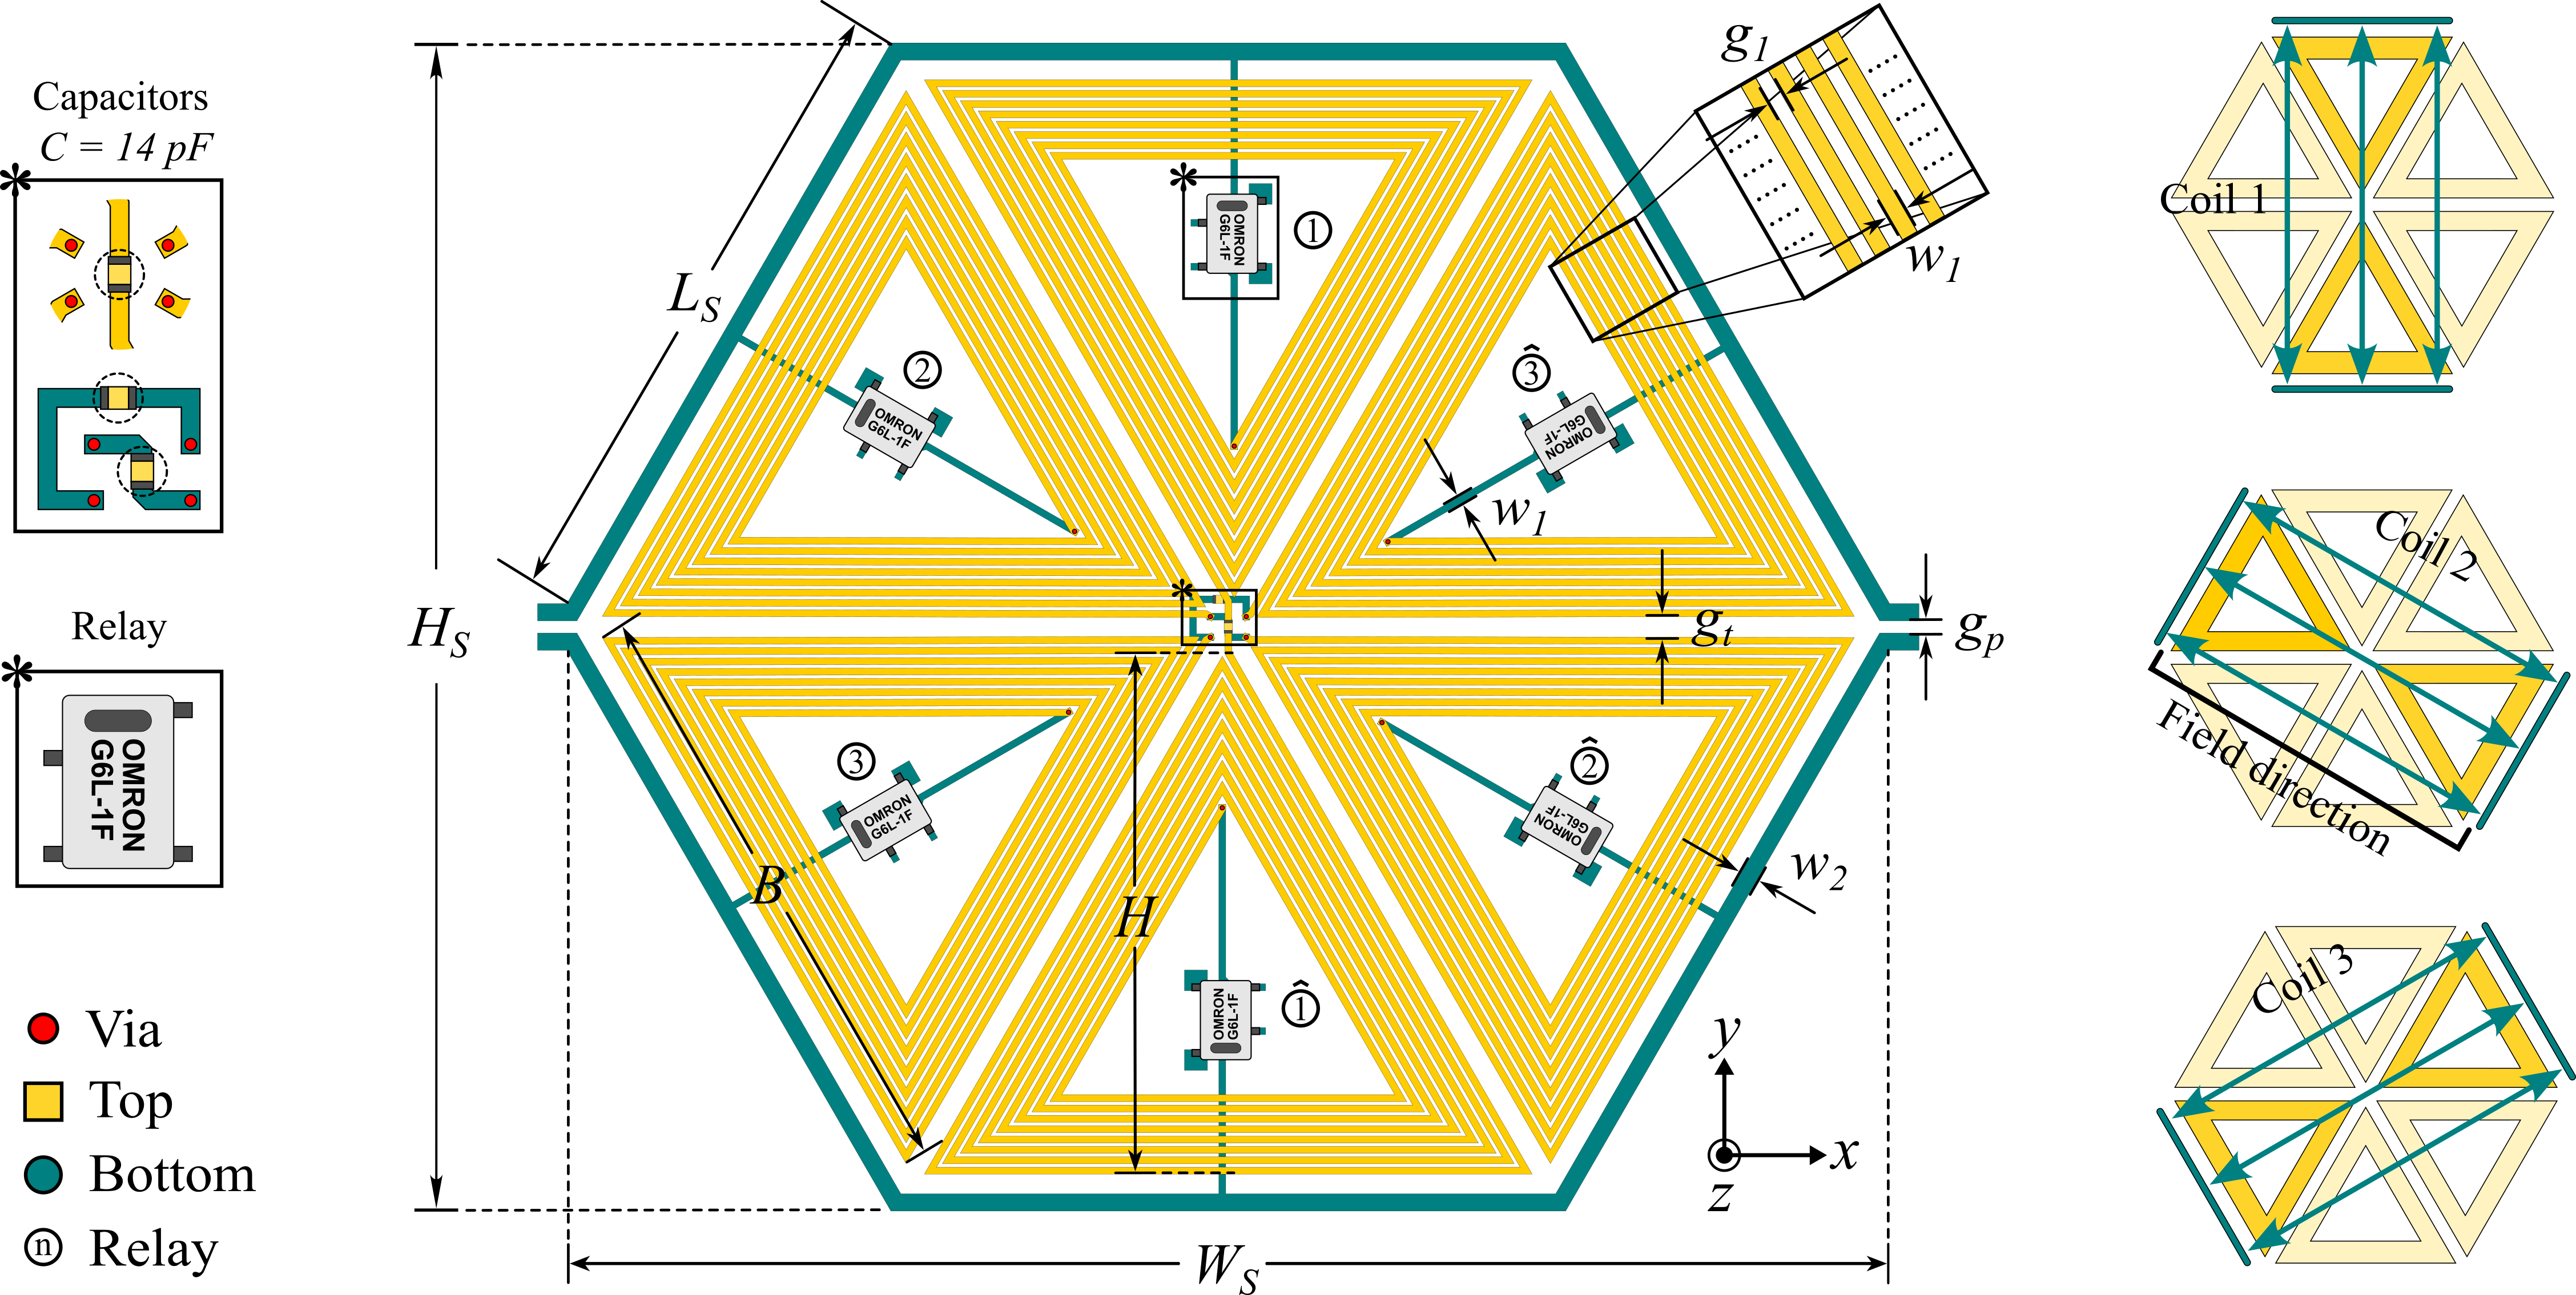
\includegraphics[width=0.95\linewidth]{t4.png}
\caption{Schematic of the proposed planar switched-coil array transmitter with three selectable coils and a relay-based switching network. The left panel shows the capacitor connections and relay configuration. The right panel highlights each individual coil and its field direction. Dimensional parameters: $H_{s}=135$~mm, $W_{s}=153$~mm, $L_{s}=75$~mm, $B=70$~mm, $H=60$~mm, $w_{1}=0.8$~mm, $g_{1}=0.4$~mm, $w_{2}=2$~mm, $g_{t}=2.3$~mm, $g_{p}=1.4$~mm, $C=14$~pF.}
\label{fig1}
\end{figure*}

\begin{figure}[!t]
\centering
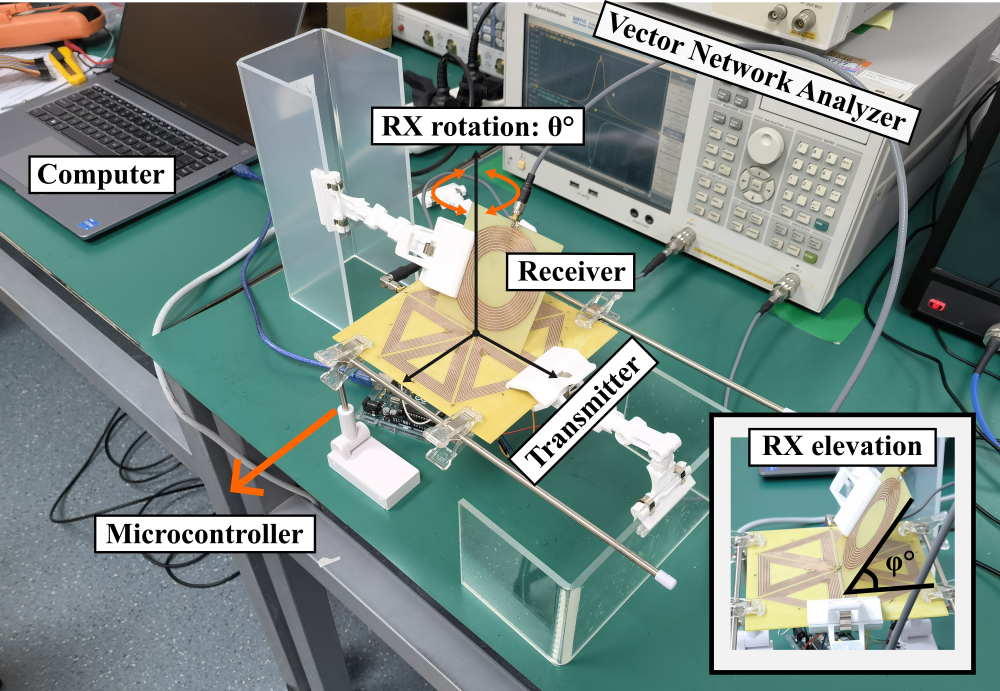
\includegraphics[width=1\linewidth]{equip.png}
\caption{Prototype and measurement setup of the proposed WPT system. The nominal vertical Rx configuration corresponds to $\phi=90^\circ$, and the Rx azimuthal rotation angle is denoted by $\theta$.}
\label{fig2}
\end{figure}

The transmitter topology of the proposed WPT system is shown in Fig.~\ref{fig1}. It consists of three triangular double-D (DD) coils and a coil-switching network. A hexagonal source loop is placed at the bottom of the transmitter and is connected to the three coils through normally open relays (Omron G6L-1F). To energize a particular coil, the two relays associated with that coil are closed, while the others remain open, so that only one Tx coil is activated at a time. The transmitter is driven by a single-channel excitation source (i.e., one port).

Because the Tx array is formed by DD coils, which create alternating N--S poles through oppositely wound spirals, the magnetic field produced by the Tx array has components parallel to the Tx plane. Based on this, the nominal Rx configuration is orthogonal to the Tx plane. As shown in Fig.~\ref{fig2}, the fabricated transmitter was clamped by two hangers, and the receiver was held by an adjustable plastic arm to allow azimuthal rotation and elevation variation.

The Rx used in this work is a planar circular coil with a diameter of 78.4~mm. The Rx coil has nine turns, with an inner radius of 20.0~mm, an outer radius of 38.2~mm, a trace width of 1.4~mm, and a trace gap of 0.7~mm. Both the Tx and Rx coils are fabricated on a 1.0~mm thick FR4 substrate.

The proposed WPT system is designed to tolerate both azimuthal rotation and elevation variation in Rx orientation. During azimuthal rotation, different Tx coils are activated in different angular regions to maintain effective power transfer. Specifically, coil~1 covers $120^\circ$--$180^\circ$ and $300^\circ$--$360^\circ$, coil~2 covers $60^\circ$--$120^\circ$ and $240^\circ$--$300^\circ$, and coil~3 covers $0^\circ$--$60^\circ$ and $180^\circ$--$240^\circ$. For elevation variation, the DD coil can naturally maintain effective coupling, because its magnetic field contains components intersecting the Rx plane when the Rx is tilted.

\begin{figure}[!t]
\centering
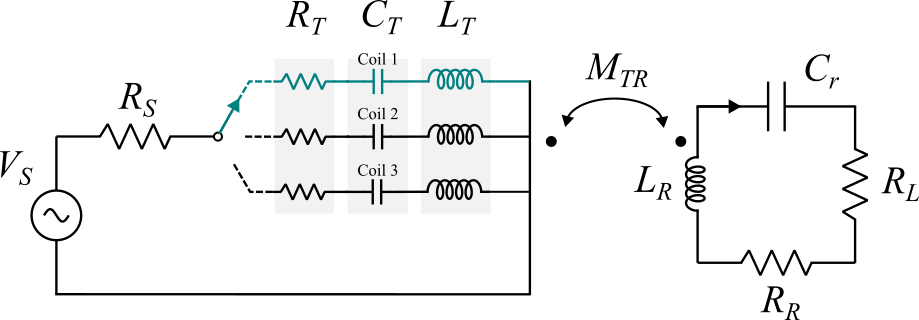
\includegraphics[width=1\linewidth]{ct1.png}
\caption{Equivalent circuit of the proposed WPT system, in which $R_{S}=50~\Omega$, $R_{T}=12.1~\Omega$, $C_{T}=14$~pF, $L_{T}=9.3~\mu$H, $L_{R}=6.9~\mu$H, $C_{R}=20$~pF, $R_{R}=2.9~\Omega$, $R_{L}=50~\Omega$, and $M_{TR}=0.41~\mu$H ($\theta=0^\circ$ and coil 1 is activated).}
\label{fig3}
\end{figure}

The equivalent circuit of the proposed WPT system is shown in Fig.~\ref{fig3}. Each Tx coil is modeled as a separate RLC branch, which includes a resonant capacitor that tunes the system operating frequency to 13.56~MHz. For each switching state, the active Tx branch and the Rx coil form a conventional two-coil WPT system with series--series (SS) compensation.

The S-parameters were measured using a vector network analyzer (Keysight E5071C), and the relay states were set by an Arduino Uno R3 microcontroller. To evaluate the performance of the proposed WPT system, the power transfer efficiency (PTE) is calculated from the measured S-parameters as follows \cite{pte1}:

\begin{equation}
\label{deqn_ex1}
\mathrm{PTE} = \frac{|S_{21}|^2}{1-|S_{11}|^2}\times100\%
\end{equation}



\section{Results and Comparison}

\begin{figure}[!t]
\centering
\subfloat[]{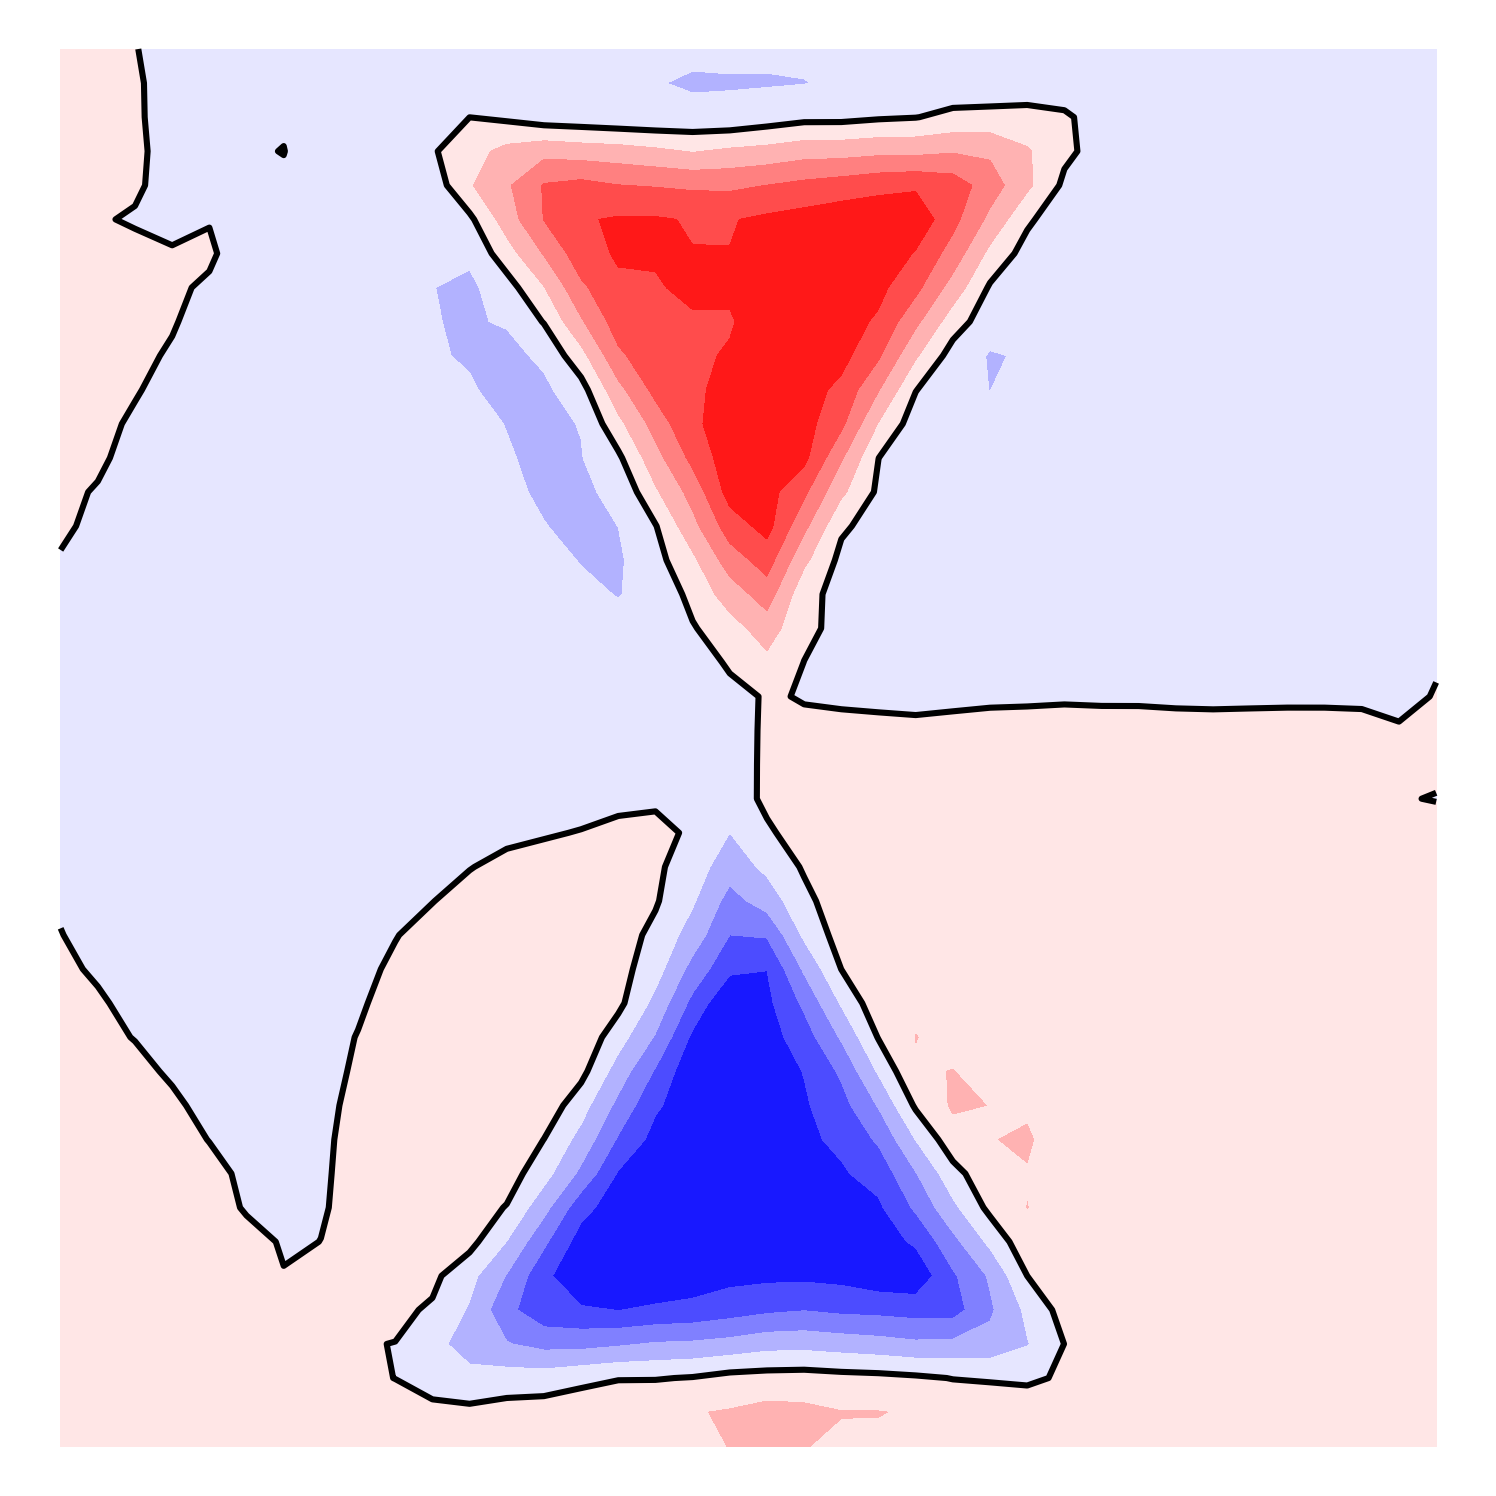
\includegraphics[width=0.33\linewidth]{field1.png}%
\label{fig4a}}
\subfloat[]{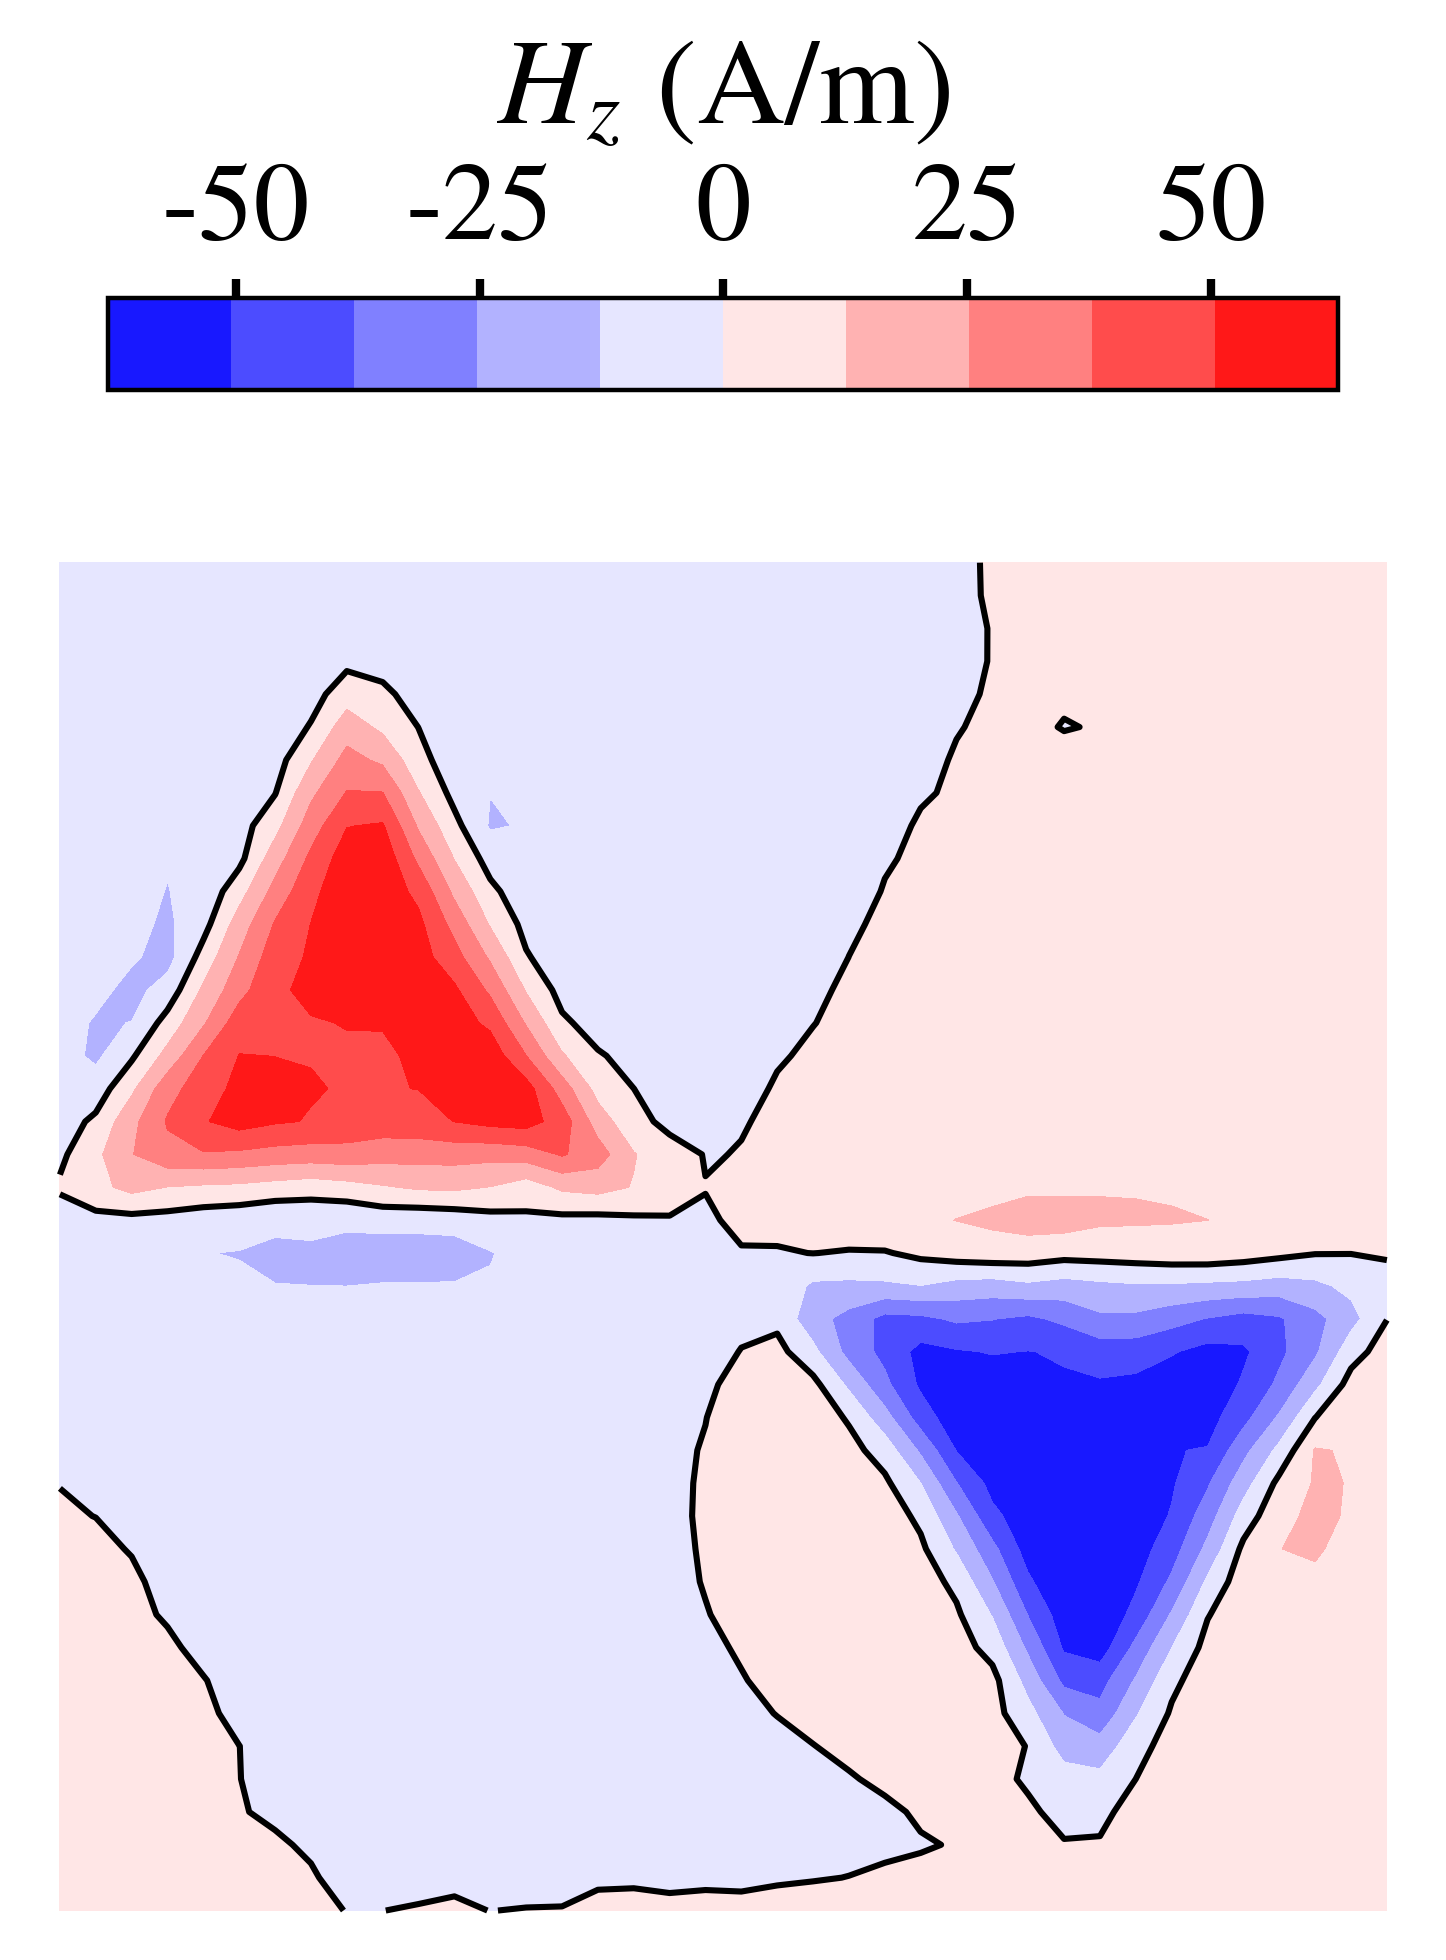
\includegraphics[width=0.33\linewidth]{field2.png}%
\label{fig4b}}
\subfloat[]{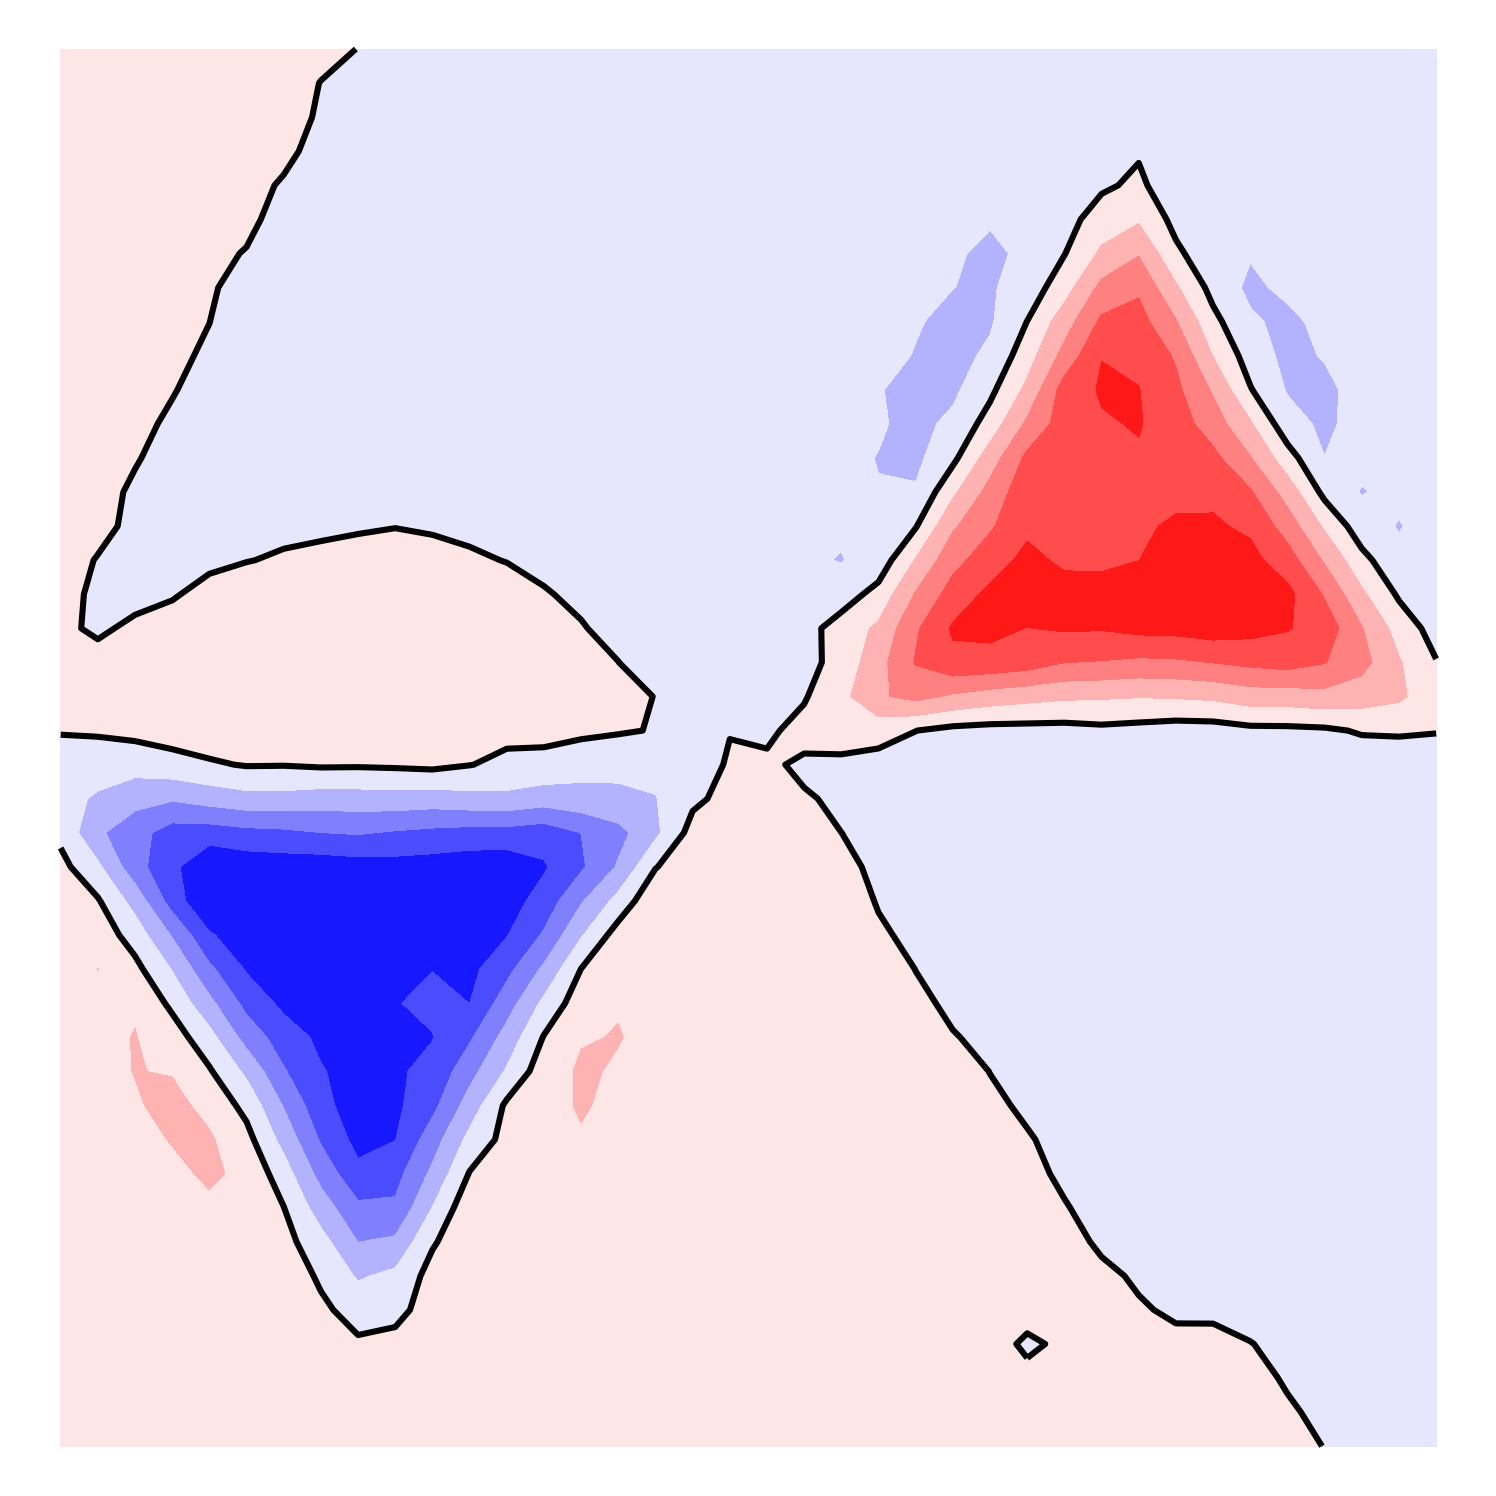
\includegraphics[width=0.33\linewidth]{field3.png}%
\label{fig4c}}
\caption{Simulated $z$\mbox{-}component magnetic field distribution for each individual coil of the proposed hexagonal array transmitter at $z=5$~mm: (a) double-D coil 1, (b) double-D coil 2, and (c) double-D coil 3.}
\label{fig4}
\end{figure}

Full-wave simulations of the hexagonal array transmitter were conducted in CST Studio Suite to evaluate the magnetic field distribution. At a height of $z=5$~mm above the transmitter plane, the $z$-component of the magnetic field strength was recorded for each coil when energized individually, as shown in Fig.~\ref{fig4}. The two spirals within each triangular double-D (DD) coil produced comparable field strengths in opposite directions, and all three cases exhibited clear N--S polarity, which preliminarily verified the intended behavior of the DD coils. The field maps also indicate that the deactivated coils do not noticeably distort the active-coil field distribution.

An azimuthal rotation experiment was performed with the vertical Rx setup ($\phi=90^\circ$). As shown in Fig.~\ref{fig6}, by switching among the three Tx coils, the proposed system maintains effective power transfer over the full azimuth range of $\theta=0^\circ$ to $360^\circ$. The measured average PTE is 66.4\%, with a maximum of 68.3\% and a minimum of 63.4\%.

\begin{figure}[!t]
\centering
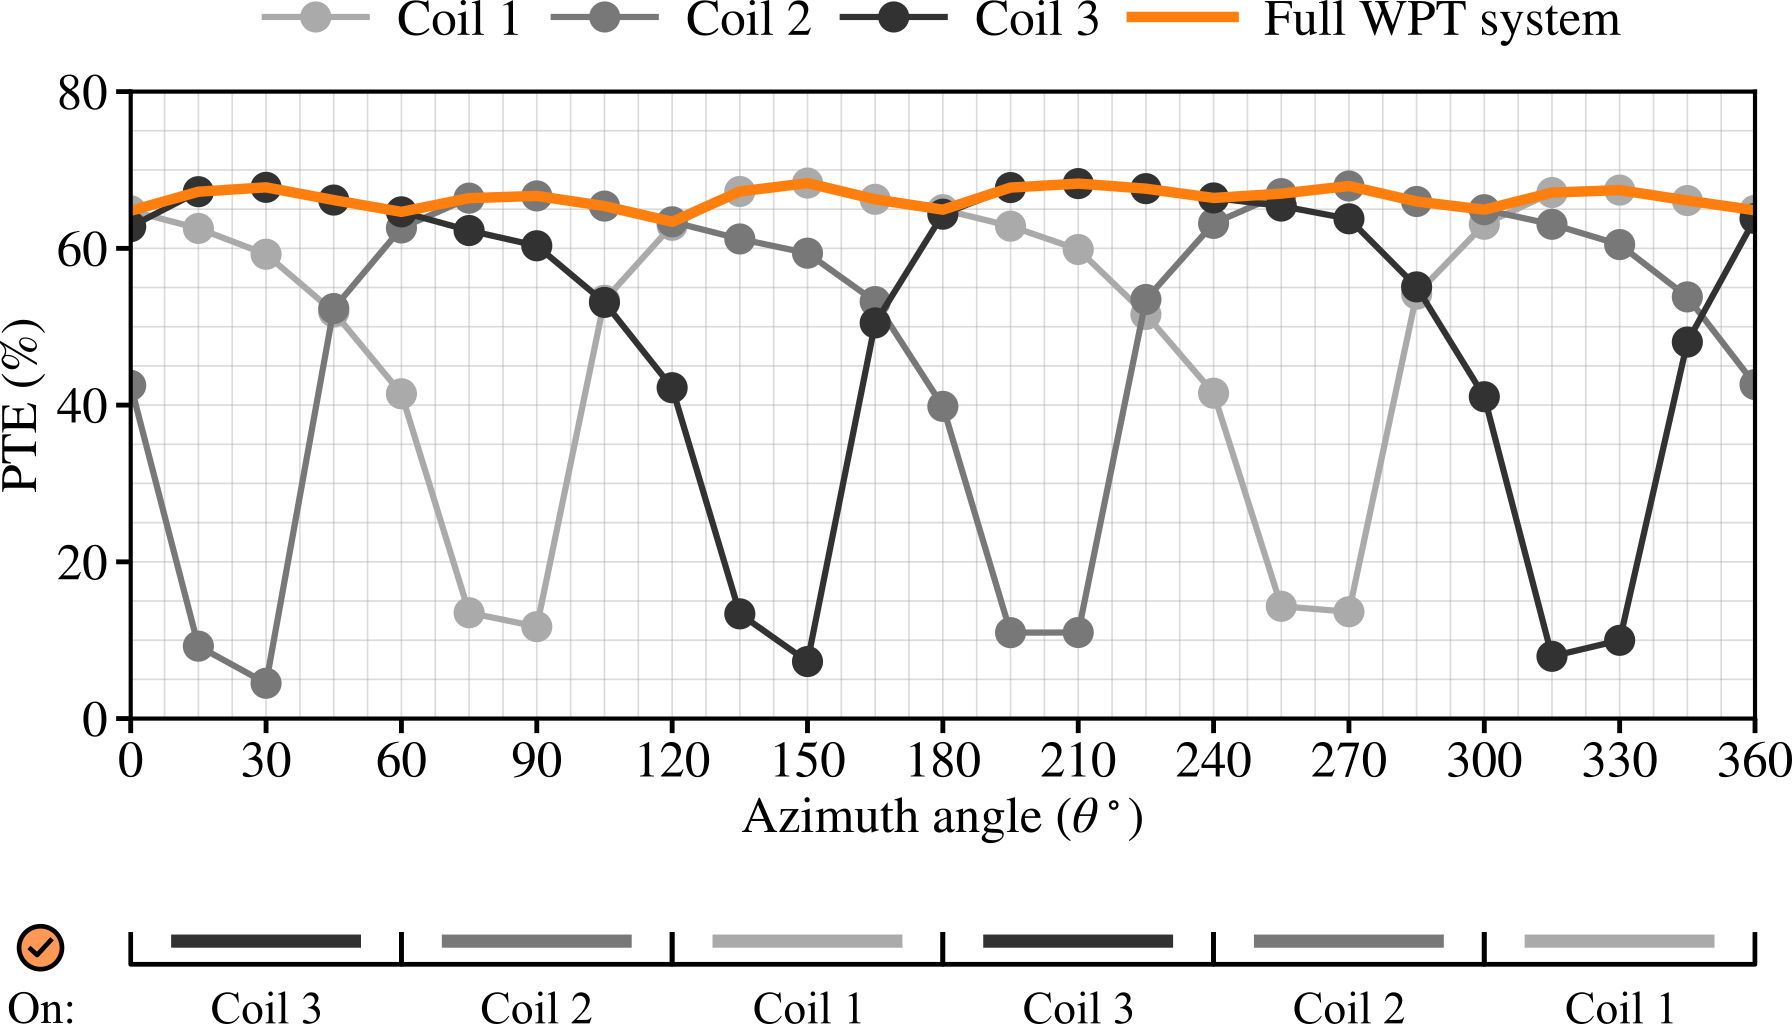
\includegraphics[width=0.85\linewidth]{R_PTE_360.png}%
\caption{Power transfer efficiency of the proposed WPT system for azimuthal rotation from $0^\circ$ to $360^\circ$ under the vertical Rx setup ($\phi=90^\circ$), together with the corresponding coil activation at different azimuth angles.}
\label{fig6}
\end{figure}
\begin{figure}
\centering
\subfloat[]{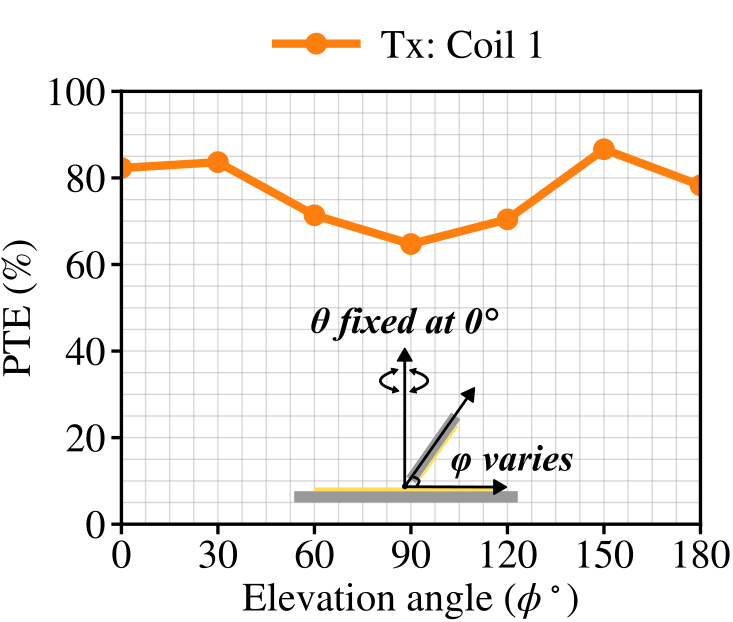
\includegraphics[width=0.42\linewidth]{E_PTE_180.png}%
\label{fig7a}}
\subfloat[]{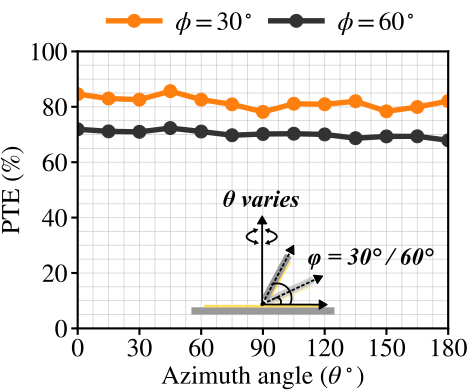
\includegraphics[width=0.42\linewidth]{RE_PTE_180.png}%
\label{fig7b}}
\caption{Power transfer efficiency of the proposed WPT system with: (a) elevation-only variation when coil 1 is activated and (b) azimuthal variation at two elevation angles ($\phi=30^\circ$ and $\phi=60^\circ$) with the full WPT system.}
\label{fig7}
\end{figure}

To investigate elevation variation, an elevation-only test was carried out under $\theta=0^\circ$ with coil 1 activated. As shown in Fig.~\ref{fig7}(a), the proposed WPT system maintains a PTE greater than 60\% for Rx elevation angles from $\phi=0^\circ$ to $180^\circ$ in increments of $30^\circ$. The lowest PTE occurs at the nominal vertical Rx position ($\phi=90^\circ$), where the measured value is about 64.7\%. This is because, as the Rx tilts away from the vertical position, part of the Rx coil moves closer to the Tx array, thereby reducing the coupling distance.


\begin{figure}[!t]
\centering
\subfloat[]{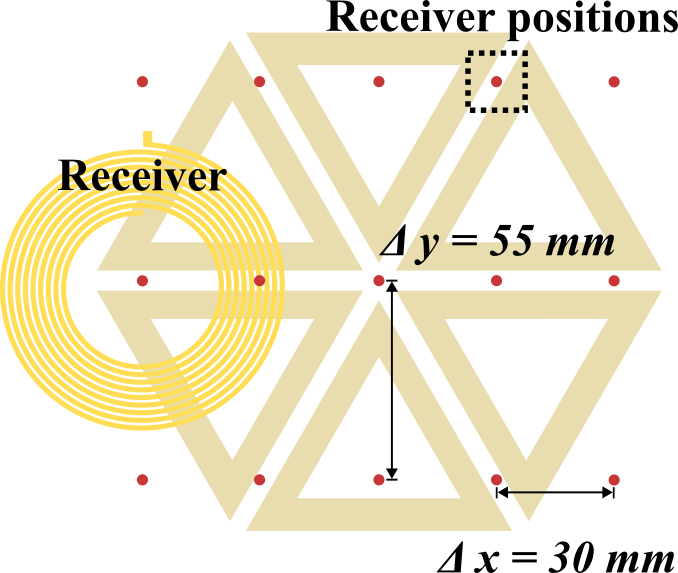
\includegraphics[width=0.4\linewidth]{lateral_rx.png}%
\label{fig8a}}
\hfill
\subfloat[]{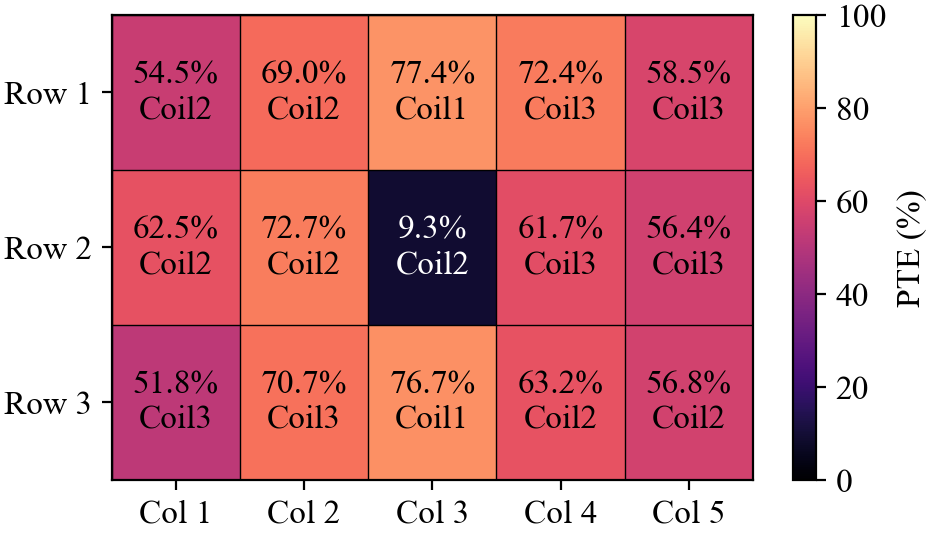
\includegraphics[width=0.6\linewidth]{Lateral_PTE.png}%
\label{fig8b}}
\caption{Lateral-position sensitivity test of the proposed WPT system: (a) measurement setup and (b) measured power transfer efficiency at different lateral positions.}
\label{fig8}
\end{figure}


Additionally, azimuthal rotation was investigated at different elevation angles, as shown in Fig.~\ref{fig7}(b). The PTE was measured over an azimuthal range of $\theta=0^\circ$ to $180^\circ$ in $15^\circ$ increments at $\phi=30^\circ$ and $\phi=60^\circ$. In both cases, the PTE remains above 65\% over the entire measured rotation range. The average measured PTE is 81.6\% at $\phi=30^\circ$ and 70.2\% at $\phi=60^\circ$, while the peak PTE reaches 85.6\% at $\phi=30^\circ$. These results indicate that the proposed WPT system can maintain orientation tolerance under different elevation conditions, and can therefore accommodate both azimuthal and elevation misalignment simultaneously.

The proposed WPT system was also tested under lateral offsets. As shown in Fig.~\ref{fig8}(a), the Rx coil was placed parallel to the Tx plane with a gap distance of 40~mm and moved to 15 positions arranged in a $3\times5$ grid. As shown in Fig.~\ref{fig8}(b), the proposed system maintains a PTE above 50\% at the farthest offset positions, indicating effective power transfer under relatively large lateral offsets. However, when the Rx coil is located at the geometric center of the Tx coil array, the measured PTE drops to 9.3\% because of the intrinsic field-cancellation effect of the DD coil structure. Therefore, the results might be interpreted as demonstrating large-offset transfer capability with a center null.


Finally, Table~\ref{tab1} compares the proposed system with recent orientation-tolerant WPT systems. The proposed system provides orientation-tolerance capability comparable to that of other recent works. However, other systems usually rely on more complex strategies. For example, \cite{consu} employs three excitation channels with amplitude modulation, and \cite{multi} adopts four-channel closed-loop phase control. These methods require multiple independent excitation channels to create rotating or targeted magnetic fields. By contrast, the proposed system requires only a single excitation channel with discrete coil selection.

\begin{table}[!t]
\centering
\footnotesize
\setlength{\tabcolsep}{4pt}
\renewcommand{\arraystretch}{2}

\caption{Comparison with other orientation-tolerant WPT systems}
\label{tab1}

\begin{threeparttable}
\begin{tabular}{cccccc}
\hline
\textbf{Ref.}  & \cite{3D} & \cite{consu} & \cite{hybrid} & \cite{multi} & \textbf{This work} \\
\hline
\hline
Year  & 2023 & 2024 & 2024 & 2024 & \textbf{2026} \\
\hline
Freq. (MHz) & 6.78 & 6.78 & 6.78 & 6.78 & \textbf{13.56} \\
\hline
Tx Dim.\tnote{1} & 3-D & 2-D & 2-D & 2-D & \textbf{2-D} \\
Rx Dim. & 2-D & 2-D & 2-D & 2-D & \textbf{2-D} \\
\hline
Method & switching & modulation & IMN\tnote{2} & phase-shift & \textbf{switching} \\
Excitation & 1 & 3 & 1 & 4 & \textbf{1} \\
\hline
Tolerance\tnote{3} & A, E & A, E & A, E & A, E & \textbf{A, E} \\
\hline
Peak $\eta$ & 71.6\% & 78\% & 80\% & 80.2\% & \textbf{68.3 / 85.6\%} \\
\hline
\end{tabular}
\vspace{0.5em}

\begin{tablenotes}
\footnotesize
\item[1] Dim. denotes dimension.
\item[2] IMN denotes the impedance-matching network.
\item[3] A and E denote azimuth and elevation tolerance, respectively.
\end{tablenotes}

\end{threeparttable}
\end{table}

In addition, \cite{3D} also adopts a coil-switching strategy, but its 3-D Tx geometry is more suitable for charging devices in idle states, whereas the proposed planar Tx is better suited to charge-while-use applications due to its open transmitter structure. Furthermore, \cite{hybrid} presents an elegant passive solution that utilizes a hybrid Tx with impedance-matching networks to achieve orientation tolerance. The hybrid Tx in \cite{hybrid} is a multilayer structure composed of a bow-tie coil, a circular coil, and a DD coil. By contrast, the proposed system uses a single-layer printed Tx array, which has a more straightforward coil design while requiring a simple switching network.



\section{Conclusion}
An orientation-tolerant wireless power transfer system based on a printed switched-coil array has been demonstrated at 13.56~MHz. Experimental results verify that the proposed system can maintain stable power transfer over the full azimuth range, while also exhibiting tolerance to elevation variation. Lateral-position measurements further show effective power transfer at large offsets, with a center null caused by the DD field distribution. These results confirm that the proposed system provides an effective orientation-tolerant WPT solution with a planar transmitter structure and coil-switching strategy.


\newpage
\begin{thebibliography}{99}
\balance


\bibitem{consumer} H. Hoang, S. Lee, Y. Kim, Y. Choi and F. Bien, ``An adaptive technique to improve wireless power transfer for consumer electronics,'' in IEEE Transactions on Consumer Electronics, vol. 58, no. 2, pp. 327-332, May 2012.

\bibitem{wearable} J. Lee, Y. Kim, D. Kang, I. Song and B. Lee, ``A Reconfigurable Bidirectional Wireless Power and Full-Duplex Data Transceiver IC for Wearable Biomedical Applications,'' in IEEE Transactions on Biomedical Circuits and Systems, vol. 19, no. 4, pp. 767-776, Aug. 2025.

\bibitem{bio} T. Campi, S. Cruciani, F. Maradei and M. Feliziani, ``Innovative Wireless Charging System for Implantable Capsule Robots,'' in IEEE Transactions on Electromagnetic Compatibility, vol. 63, no. 5, pp. 1726-1734, Oct. 2021.

\bibitem{ev} Z. Deng et al., ``Design of a 60-kW EV Dynamic Wireless Power Transfer System With Dual Transmitters and Dual Receivers,'' in IEEE Journal of Emerging and Selected Topics in Power Electronics, vol. 12, no. 1, pp. 316-327, Feb. 2024.

\bibitem{geo1} S. Wang, Z. Hu, C. Rong, C. Lu, J. Chen and M. Liu, ``Planar Multiple-Antiparallel Square Transmitter for Position-Insensitive Wireless Power Transfer,'' in IEEE Antennas and Wireless Propagation Letters, vol. 17, no. 2, pp. 188-192, Feb. 2018.

\bibitem{geo3} Y. Zhuang, A. Chen, C. Xu, Y. Huang, H. Zhao and J. Zhou, ``Range Adaptive Wireless Power Transfer Based on Differential Coupling Using Multiple Bidirectional Coils,'' in IEEE Transactions on Industrial Electronics, vol. 67, no. 9, pp. 7519-7528, Sept. 2020.

\bibitem{geo4} D. Vital and S. Bhardwaj, ``Misalignment Resilient Anchor-Shaped Antennas in Near-Field Wireless Power Transfer Using Electric and Magnetic Coupling Modes,'' in IEEE Transactions on Antennas and Propagation, vol. 69, no. 5, pp. 2513-2521, May 2021.

\bibitem{ar3} S. A. Mirbozorgi, H. Bahrami, M. Sawan and B. Gosselin, ``A Smart Multicoil Inductively Coupled Array for Wireless Power Transmission,'' in IEEE Transactions on Industrial Electronics, vol. 61, no. 11, pp. 6061-6070, Nov. 2014.

\bibitem{ar4} J. Li, N. Kou, S. Yu, Z. Ding and Z. Zhang, ``Reconfigurable PCB Coil Array Loaded With PIN Diodes for Improving Transmission Efficiency in MCR-WPT Systems,'' in IEEE Antennas and Wireless Propagation Letters, vol. 22, no. 7, pp. 1667-1671, July 2023.

\bibitem{3drx1} Z. Zhang and B. Zhang, ``Angular-Misalignment Insensitive Omnidirectional Wireless Power Transfer,'' in IEEE Transactions on Industrial Electronics, vol. 67, no. 4, pp. 2755-2764, April 2020.


\bibitem{3drx3} A. Basir, I. A. Shah and H. Yoo, ``Sphere-Shaped Receiver Coil for Misalignment-Resilient Wireless Power Transfer Systems for Implantable Devices,'' in IEEE Transactions on Antennas and Propagation, vol. 70, no. 9, pp. 8368-8378, Sept. 2022.


\bibitem{3drx5} S. R. Khan, S. K. Pavuluri, G. Cummins and M. P. Y. Desmulliez, ``Miniaturized 3-D Cross-Type Receiver for Wirelessly Powered Capsule Endoscopy,'' in IEEE Transactions on Microwave Theory and Techniques, vol. 67, no. 5, pp. 1985-1993, May 2019.


\bibitem{comp2} Z. Liu et al., ``A Misalignment Resilient System for Magnetically Coupled Resonant Wireless Power Transfer,'' in IEEE Transactions on Antennas and Propagation, vol. 68, no. 12, pp. 8260-8265, Dec. 2020.


\bibitem{bowl} J. Feng, Q. Li, F. C. Lee and M. Fu, ``Transmitter Coils Design for Free-Positioning Omnidirectional Wireless Power Transfer System,'' in IEEE Transactions on Industrial Informatics, vol. 15, no. 8, pp. 4656-4664, Aug. 2019.

\bibitem{3D}
S. -Y. Kim, N. -R. Kwon, S. -H. Ahn and W. -S. Lee, ``Three-Dimensional Wireless Power Transfer System Using Multiple Orthogonal Resonators for Spatial Freedom,'' in IEEE Transactions on Antennas and Propagation, vol. 71, no. 5, pp. 4036-4044, May 2023.

\bibitem{consu}
X. Yu, J. Feng, L. Zhu and Q. Li, ``Design and Optimization of a Planar Omnidirectional Wireless Power Transfer System for Consumer Electronics,'' in IEEE Open Journal of Power Electronics, vol. 5, pp. 311-322, 2024.

\bibitem{multi}
N. Kang, H. Qin, R. Ma, C. H. T. Lee, M. Liu and C. Ma, ``Magnetic Field Projection and Current Phase Control in a 2-D Planar Transmitting Coil Array,'' in IEEE Transactions on Power Electronics, vol. 39, no. 9, pp. 10623-10637, Sept. 2024.

\bibitem{pte1}
H. Le-Huu, G. T. Bui and C. Seo, ``Efficient Compact Radiative Near-Field Wireless Power Transfer to Miniature Biomedical Implants,'' in IEEE Antennas and Wireless Propagation Letters, vol. 22, no. 12, pp. 2803-2807, Dec. 2023.

\bibitem{hybrid}
H. Le-Huu and C. Seo, ``A Hybrid Transmitting Coil for Improving Angular Freedom of a Wireless Power Transfer System,'' in IEEE Microwave and Wireless Technology Letters, vol. 34, no. 1, pp. 119-122, Jan. 2024.



\end{thebibliography}


\end{document}
